\documentclass[11pt]{article}
\usepackage{fontspec}
\setmainfont{TeX Gyre Pagella}
\usepackage[a4paper,margin=1.1in]{geometry}
\usepackage{amsmath,amssymb}
\usepackage{booktabs}
\usepackage{tikz}
\usetikzlibrary{positioning}
\usepackage{microtype}
\usepackage[hidelinks]{hyperref}
\usepackage{setspace}
\onehalfspacing
\setlength{\parskip}{0.4em}

\title{Consistency Constraints and the Geometry of Learned Representations}
\author{Flyxion\\Independent Researcher}
\date{July 2026}

\begin{document}
\maketitle

\begin{abstract}
Foundation models learn almost entirely from text. This is usually treated as a fact about data availability rather than as a design decision, and the question of whether text is a good substrate on which to build foundational representations is rarely asked. This paper proposes that the relevant design variable is neither the modality nor the language of a curriculum but the consistency constraints it imposes: the extent to which a learner is required to reconcile multiple partially independent observations of a shared latent state. We state this as the Representational Constraint Hypothesis, define a measure of constraint diversity over the observation channels a curriculum supplies, and give conditions under which such constraints are informative rather than spurious. Several independent research directions are then legible as instances of one principle, among them contrastive multimodal pretraining, transfer from structured non-linguistic data, and the Basque First hypothesis of Eichler, who identifies redundancy rather than morphological richness as the operative property of his proposed curriculum and to whom the mechanism developed here is directly indebted. Generalizing that identification beyond a single symbolic channel yields a two-dimensional space of curricula whose coordinates are symbolic explicitness and constraint diversity, in which existing proposals occupy different regions and one region is occupied by none. We examine signed language as the richest naturally occurring high-diversity curriculum, specify an experimental program that varies both coordinates independently, and identify a synthetic embodied substrate as the curriculum the framework predicts but no current proposal develops.
\end{abstract}



\section{The Hidden Assumption}
\label{sec:assumption}

Large language model development has been optimized aggressively along several axes. Compute has been scaled by orders of magnitude, data volume with it. Tokenization schemes, positional encodings, attention variants, optimizer schedules, and alignment procedures have each received sustained attention. Underneath all of this sits a choice that is almost never treated as a choice at all: that a foundation model should learn, first and predominantly, from written text.

The reasons for this are practical rather than principled. Text is abundant, cheap to store, easy to tokenize, and already digitized at a scale no other modality approaches. Nothing about that list is an argument that text is a good substrate on which to build representations. It is an argument that text is an available one. The distinction matters because the two questions have different answers, and only the first has been asked.

There is a temptation to reframe the question as one about which natural language should be used, and this reframing is a mistake worth naming early. Languages are interfaces. They are shaped by the histories and purposes of their speakers, and asking which of them has the best grammar for thought is close to a category error, in the same way that asking whether Cartesian or spherical coordinates are correct is a category error: each is adapted to certain structures and awkward for others, and neither is intrinsically prior. English is not dominant in training corpora because it is well suited to reasoning. It is dominant because it has been used across an unusually wide range of domains and therefore accumulated an unusually large written record.

The question this paper asks is different, and it survives the interface objection. Rather than asking which language or which modality a learner should encounter first, it asks what structural property of a curriculum makes early exposure consequential at all. The answer proposed here is that curricula matter to the extent that they require the learner to reconcile several partially independent views of the same underlying state, and that this property is measurable, is largely orthogonal to the identity of the language or modality supplying it, and is close to absent from text-only pretraining.

\section{What Makes a Foundational Curriculum Consequential}
\label{sec:hypothesis}

We state the proposal directly before motivating it.

\textbf{The Representational Constraint Hypothesis.} Foundational curricula exert their greatest influence on learned representations when they require a model to reconcile multiple independent views of the same underlying state. The resulting latent variables become organized around invariants that persist across those views rather than around statistics peculiar to any single view. The number and independence of these views, not the channel in which they are expressed, is the quantity that curriculum design should control.

The reasoning is straightforward. Consider a learner exposed to two or more channels that each depend on a common latent state through distinct and only partially correlated noise processes. A representation that overfits to any single channel will fail to predict the others, so only a representation capturing what the channels share will generalize across them. Agreement between independently corrupted or independently projected observations thereby functions as a supervisory signal for invariant structure without any invariant needing to be specified in advance. A single channel supplies no such signal, because there is nothing against which its account can be checked.

This is a claim about supervision rather than about richness. A curriculum can be enormously rich within one channel and still supply the learner with exactly one account of each state. What distinguishes a constraint from a cue is that a constraint must be satisfied jointly, and joint satisfaction is what forces the learner toward the latent variable through which the channels are related. Where a cue may or may not be exploited, a constraint has to be reconciled to predict either channel from the other.

Stated this way the hypothesis makes no reference to language, modality, or embodiment. Vision and proprioception are independent views of a reaching movement. An image and its caption are independent views of a scene. Two morphological systems marking the same grammatical relation are independent views of that relation. In each case the learner faces the same demand, and the hypothesis predicts the same consequence.

\section{Why Foundational Training Is Privileged}
\label{sec:early}

The hypothesis of the previous section concerns curricula, but it carries an unstated assumption that deserves its own argument: that when constraints arrive matters, and that constraints imposed early do something constraints imposed later do not. Without that assumption the proposal collapses into a claim about training data composition, and the natural objection follows immediately. If cross-channel consistency is valuable, why not introduce it midway through pretraining, or at the end, where the engineering is easier and the data requirements less severe?

We think there is a specific answer, and that it is stronger than an appeal to analogy with biological critical periods. It should be flagged plainly as a conjectured mechanism about optimization dynamics rather than an established result: it follows from a general intuition about what gradient descent finds cheapest, not from a proof about transformer training in particular, and the prediction below states the experiment that would confirm or disconfirm it.

\subsection{The Translation Shortcut Hypothesis}

We call this the Translation Shortcut Hypothesis. A consistency constraint can be satisfied in two ways. The learner can organize a shared latent representation in which both channels are expressed, so that agreement between them is a consequence of the representation rather than something separately enforced. Or the learner can maintain separate channel-specific representations and learn a mapping between them, so that agreement is produced by translation at the point where the constraint is applied. Both satisfy the objective. Only the first produces the representational reorganization the hypothesis is about.

Which solution a learner finds depends on what it already has. A model that has trained extensively on a single channel arrives at the moment of constraint imposition with a working, highly optimized representation of that channel and no particular pressure to disturb it. The cheapest path to satisfying a newly added constraint is then to attach a mapping between the existing representation and the new channel, since this leaves the expensive and already functional structure intact. Gradient descent is not indifferent between these solutions; it takes the one requiring the smaller change, and late in training the smaller change is the translation layer.

A model that encounters the channels together from the beginning has no such option, because there is no working single-channel representation for a translation layer to attach to. The only representations available are ones being built under the constraint, and a representation that satisfies the constraint structurally is not more expensive than one that does not, since neither exists yet. The asymmetry is therefore not about plasticity in the abstract but about the availability of a shortcut, and the shortcut becomes available exactly when a competent single-channel solution has been established.

\subsection{Coordinate Systems and Their Elaboration}

A second consideration reinforces the first and is closer to how representations are actually reused. Features learned later in training are largely composed from features already present, so early representations function less like a set of learned facts than like a coordinate system in which subsequent distinctions are expressed. A distinction that has no compact expression in that coordinate system does not become impossible to represent, but it becomes expensive: it must be assembled from combinations of an ill-suited basis rather than read off directly, and gradient descent will find the assembly before it will find a reorganization of the basis.

This is the sense in which the ordering matters even where final aggregate performance does not differ. Two models can converge to similar loss while representing the same distinctions in bases of very different suitability, and the difference shows up not in the training objective but in what transfers, what is linearly recoverable, and what can be learned quickly downstream. The controlled ordering studies that find equivalent final benchmark performance alongside different learning trajectories and representational geometry are consistent with exactly this picture, and they are a caution about experimental design rather than evidence against the hypothesis.

There is a mechanical contributor as well. Learning rate schedules decay, and the magnitude of the updates available late in training is smaller than what a reorganization of the representational basis would require. This does not create the asymmetry, but it deepens it, since the shortcut becomes not merely cheaper but the only change the optimizer is still in a position to make.

\subsection{A Second Testable Prediction}
\label{sec:shortcut-prediction}

The shortcut argument is worth stating carefully because it is falsifiable independently of the main hypothesis, and it is falsifiable with the instruments already required by the experimental design.

If constraints imposed late are satisfied by translation while constraints imposed early are satisfied structurally, then the two should differ in where in the network cross-channel binding occurs. A model trained on multiple channels from the outset should bind them in early and middle layers, since the shared representation is what the later layers are built on. A model that acquires a second channel after extensive single-channel training should bind them late, near the point where the constraint is applied, leaving its earlier layers substantially unchanged. Depth of binding is measurable by the same probing and attention-specialization methods used to assess representational geometry, and it does not require waiting for downstream task results.

The prediction is sharper than the main hypothesis because it can fail in an informative way. If late-constrained models turn out to reorganize their early layers after all, then the shortcut argument is wrong, the timing assumption is unsupported, and the practical recommendation changes from curriculum design to data composition, which would be a considerably cheaper conclusion for the field. If early and late constraint imposition produce indistinguishable binding depth and indistinguishable geometry, the case for foundational curricula as a distinct research direction is substantially weakened regardless of what benchmark scores show.


\section{Convergent Evidence}
\label{sec:convergent}

Several research directions that are not usually discussed together become legible as instances of this principle, and their independence from one another is part of the evidence. None was designed to test the hypothesis stated above; that they point in a common direction is therefore informative.

Contrastive multimodal pretraining uses agreement between paired observations as its training signal. Aligning images with captions, or aligning augmented views of one input, produces representations organized around what the views share, and does so without labeled invariants. This is the hypothesis operating as an explicit objective, though it is generally presented as a technique for learning transferable features rather than as a claim about curricula.

Transfer from structured non-linguistic data supplies a second line. Papadimitriou and Jurafsky (2020) showed that pretraining on music, code, and nested symbolic sequences transfers measurable structural bias to subsequent language modeling. This result is difficult to accommodate on any account in which the identity of the first natural language is the operative variable, since the first material is not a natural language at all. Hu et al. (2025) found that pre-pretraining on formal languages with hierarchical structure improves later natural-language learning, with structured artificial tokens proving worth more, token for token, than natural ones, and reported a non-monotonic dose curve in which benefit reverses beyond an optimal duration. Shinnick et al. (2025) found that transformers pretrained on procedural data develop modular internal structure for algorithmic reasoning. Each establishes that what a model trains on first shapes what it learns later; none offers a mechanism for why.

Curriculum learning in its standard form sequences examples by difficulty within a fixed distribution, which is a different variable, but recent controlled work varying only data order finds that ordering acts as a selective inductive bias, reshaping representational geometry and learning dynamics even where final aggregate accuracy is unchanged. That dissociation between geometry and benchmark performance recurs below and constrains how any test of the present hypothesis must be designed.

\subsection{The Closest Precedent}

One proposal in this literature identifies the constraint property explicitly as the mechanism, and it deserves more than equal weight among the foregoing because it is the one place where the hypothesis of this paper has been independently arrived at, albeit in a restricted form.

Eichler's Basque First hypothesis argues that English-first pretraining builds reasoning capacity on a morphologically impoverished foundation, encoding argument structure through positional heuristics rather than explicit grammatical marking, and proposes beginning with a typologically distant, morphologically rich language instead. Read as a claim about Basque, the proposal is vulnerable to the interface objection of Section~\ref{sec:assumption}: it is not obvious why any particular natural language should be a privileged substrate for machine reasoning. But the paper's own justification for selecting Basque is not richness. Basque marks predicate-argument structure twice, by case on the argument and by polypersonal agreement on the verb, and Eichler identifies this redundancy rather than morphological richness as the mechanistically important property, on the grounds that a single explicit encoding gives the model a cue it may or may not exploit while a doubled encoding gives it a consistency constraint, since the two markings are recoverable from each other and must be reconciled to predict either one. He describes this as closer to supervision of the structure than to a distributional hint at it.

That is the Representational Constraint Hypothesis, stated for the case of two morphological systems within one written channel. The present paper is indebted to it and claims no priority over it. Two further features of the Basque First proposal support reading it this way rather than as a claim about a preferred language. Its trajectory does not terminate in Basque but in a synthetic training language designed to encode logical structure without the accidents of natural language, and a proposal that regarded Basque as privileged would not propose to discard it. And its stated open question is whether early structure survives the volume of later training, which is a question about foundational geometry rather than about linguistic identity.

\subsection{Two Objectives, Not One}

Recognizing the shared mechanism also exposes a divergence, and this divergence organizes much of what follows.

Eichler's program moves from English through Basque toward a synthetic logical language of maximal explicitness, in which predicate-argument structure, evidentiality, quantifier scope, and entailment are all marked overtly and nothing is left to pragmatic inference. Each step removes ambiguity from a single channel. The direction this paper pursues instead adds channels: speech constraining text, signed language distributing one relation across several simultaneous articulators, embodied interaction supplying vision, pose, contact, and outcome as views of a shared physical event. Each step increases the number of simultaneous consistency conditions without necessarily making any of them more explicit.

These are different objectives and they are not obviously equivalent. A perfectly explicit symbolic language minimizes ambiguity within its channel while supplying exactly one account of each state, so there is nothing for the learner to reconcile. A multimodal curriculum may leave every individual channel ambiguous while supplying many partially redundant accounts whose agreement carries the structural signal. Eichler's own reasoning, that a doubled encoding outperforms a single explicit one because a constraint is stronger than a cue, suggests that redundancy does work explicitness alone does not, which raises the question of whether a maximally explicit single channel forfeits the very property he identified. Whether the two objectives coincide, trade off, or contribute independently is an empirical question, and Section~\ref{sec:experiment} is designed to answer it.


\section{The Developmental Argument, and Its Limits}
\label{sec:development}

The hypothesis of Section~\ref{sec:hypothesis} is a computational claim and must stand on computational grounds; this section adds a parallel line of evidence from human development without asking it to bear more weight than it can. Human development is not confirmation of the Representational Constraint Hypothesis, since a claim about transformer training dynamics cannot be established by facts about children. It is an existence proof of a narrower kind: at least one class of general intelligence acquires its foundational representations under a curriculum dominated by perception and action, with fluent symbolic language layered on top of an already structured sensorimotor model rather than serving as its base. That the only intelligence available for study develops in this order does not show that artificial systems must, but it does shift the burden of argument away from the assumption, currently the default, that text is the natural place to begin.

\subsection{What Precedes Language}

Before an infant produces or comprehends words, sensorimotor engagement with the world has already built a substantial model of it. Piaget's account of the sensorimotor period, whatever the fate of its finer stage boundaries under later scrutiny, established the durable observation that early cognition is organized around action schemes, reaching, grasping, tracking, whose coordination yields an understanding of objects as persisting independently of immediate perception, itself constructed through repeated manipulation across multiple sensory channels rather than given by instruction. The social prerequisites of language follow the same timetable: gaze following and joint attention emerge in the first year, well before productive speech, and become the scaffolding for reference itself, since a child learns what a word points to by first being able to follow where a caregiver is pointing. Language attaches labels and combinatorial structure to a model the child has already largely built by acting, rather than installing that model.

A parallel line in cognitive science holds that the resulting representations remain grounded in sensorimotor structure even in the mature system. Barsalou's perceptual symbol systems propose that concepts are represented in modal, perception-derived form; Lakoff and Johnson argue that abstract reasoning is structured by schemas drawn from bodily experience of space, force, and movement. Whatever the disputed details, both share the developmental record's implication: structure acquired through perception and action is not scaffolding discarded once symbols arrive but the substrate symbolic competence continues to rest on.

\subsection{What the Analogy Does Not License}

The temptation is to conclude that artificial systems should therefore be trained in the same order, and three disanalogies bound how far that conclusion travels. Human infants bring strong innate priors and maturational constraints specific to a biological agent, so it is unclear how much of the sensorimotor-first ordering reflects an optimal curriculum rather than the order in which a developing body happens to make data available. The mechanism proposed in Section~\ref{sec:hypothesis}, cross-channel consistency as a supervisory constraint, is consistent with the developmental record but not isolated by it, since human development varies many things at once and cannot be run as a controlled ablation. And the record is silent on the explicitness question that distinguishes this proposal from Eichler's, since it supplies no case in which a synthetic, maximally explicit substrate was tried instead.

The developmental argument is accordingly subordinated to the computational one. Its function is to remove the appearance of naturalness from text-first training, not to supply evidence beyond that. The claim that perception-and-action-first ordering benefits a transformer, and the reason offered for why, remain to be established by the experiments of Section~\ref{sec:experiment}.


\section{Embodied Communication}
\label{sec:embodied}

Before considering signed language it is necessary to treat the communicative behaviors that precede language and that are not linguistic at all, both because they establish the constraint-diversity axis independently of any language and because failing to separate them from signed language is the most common error in discussions of the present kind.

Pointing, gaze direction, joint attention, object manipulation in shared activity, and the imitation of another agent's action are structured communicative behaviors without grammar. They are nonetheless rich in the property this paper concerns. A pointing gesture in a shared scene supplies simultaneous constraints through the direction of the arm, the direction of gaze, the position of the body, and the referential structure of the surrounding activity, and these constrain one another through the referent rather than independently. An act of manipulation observed by a learner supplies vision, the trajectory of motion, the configuration of contact, and the resulting change in the world, all of which are views of one event and are mutually predictable only by way of that event.

These behaviors matter to the argument for a reason beyond their developmental priority. They demonstrate that constraint diversity is available without linguistic structure of any kind, which means the axis this paper proposes is not a disguised claim about which languages are best. A curriculum of manipulation and observation, containing no language, occupies a position on the diversity axis that no text corpus can reach. The claim that follows is not that signed language is superior to written language but that channels that are not language at all can supply the property Eichler identified within language.

\section{Gestural Language and the Limits of the Category}
\label{sec:gestural}


\subsection{How Far the Category Extends}

Before treating signed language it is worth asking how wide the class of gestural channels is, since the answer is less obvious than it appears and the criterion of Section~\ref{sec:constraint} settles it in a way that is worth stating in advance.

A generous reading would include mimicry, tool use, the reading of faces, and, since they are motor acts producing symbols, handwriting and typing. The first three belong in the class for the reasons given above. The last two do not, and the reason they do not is instructive. When a writer types the word for an animal, the trajectory of the fingers is fixed by the keyboard layout and carries no information about the animal. The motor channel is recoverable from the text channel by a simple mapping that has nothing to do with the referent, which is precisely the case the minimality condition of Section~\ref{sec:constraint} excludes: a simpler variable screens off the correlation, so the apparent constraint is a surface regularity. Cursive is a marginal improvement, since handwriting carries some information not present in the orthography, but the correlation between the motor trajectory and the content of the text remains screened off by the orthography itself.

Photographs and video of people acting pass the same test cleanly. The visual appearance, the pose trajectory, the configuration of contact, and the resulting change in the world are jointly constrained by the physical event and are not recoverable from one another by any fixed mapping. It is tempting to conclude that such material should therefore be classified as language, and we resist this. The framework developed here is neutral on what counts as language, and that neutrality is a feature: the question it asks is what constraints a curriculum imposes, and the answer does not change according to whether the channels are linguistic. Extending the category would purchase nothing the formalism does not already supply, while inviting a dispute about definitions in place of one about mechanisms.

\subsection{Signed Language}

American Sign Language occupies an unusual position in this space, and the reason is not that it is visual or that it involves the body. It is that ASL is a fully grammatical natural language, with phonological structure, morphology, and syntax, whose grammar is realized across several simultaneous channels rather than serialized into one. This distinguishes it sharply from the communicative behaviors of the previous section, and any treatment that assimilates signed language to gesture both misdescribes the linguistics and weakens the argument.

The parallel to Basque is more specific than simultaneity. Eichler's mechanism requires that channels be partially predictive of one another, so that predicting one constrains the other and neither can be recovered without the relation they jointly encode. Signed language satisfies this description channel by channel. Handshape constrains lexical identity. Movement constrains event structure and aspect. Location in signing space constrains referential identity, since referents are established at spatial loci and subsequently indexed there. Orientation and the path of agreement verbs constrain the assignment of grammatical roles, marking source and goal in the geometry of the sign itself rather than by position in a string. Non-manual markers, principally facial expression and head position, constrain illocutionary force, distinguishing interrogatives, conditionals, and topic marking. Body orientation constrains discourse perspective, including the attribution of reported speech and viewpoint through role shift.

These channels are neither independent nor identical, which is exactly the condition Section~\ref{sec:constraint} requires. Handshape does not determine facial expression, so the channels are separately observable. But a well-formed utterance constrains all of them jointly through the proposition being expressed, so predicting one from another requires reconstructing that proposition. This is the same structure as Basque double marking, in which case and agreement are separately observable but mutually recoverable only through the predicate-argument relation, differing in that the channels are sensorimotor rather than morphological and that there are more of them.

The consequence for the paper's thesis is deflationary in the right way. ASL is valuable here as the richest naturally occurring, fully grammatical instance of a high-diversity curriculum, which makes it the best available existence proof that human language does not require the single-channel serialization that written text imposes. It is not proposed as an optimal training substrate, and nothing in the argument depends on its being one. Its role is to demonstrate that the diversity axis extends into language proper, rather than being confined to the non-linguistic channels of the previous section.


\section{Curriculum Design as Constraint Selection}
\label{sec:constraint}

Section~\ref{sec:hypothesis} stated the hypothesis and Section~\ref{sec:convergent} showed that several independent lines of work instantiate it. This section makes the proposal precise. We hold that foundational curriculum design is best understood not as the selection of a language, a modality, or a domain, but as the selection of consistency constraints: the choice of what a learner must reconcile during the period in which its representational geometry is established. Language, modality, and domain are the vehicles through which constraints are delivered. The constraints themselves are the operative variable, and they can be defined, measured, and optimized independently of the vehicle.

\subsection{Curricula as Channel Collections}

Let $Z\in\mathcal{Z}$ denote the hidden variable that jointly explains the observations a curriculum supplies, defined by that role rather than by any prior commitment about what it is. What plays the part of $Z$ varies with the curriculum: in a written utterance it may be the predicate-argument relation, in a filmed action the event and its physical configuration, in a manipulation episode the state of the objects handled. These are examples of the role, not distinct senses of the symbol, and the formalism below is indifferent among them. A curriculum stage supplies a collection of observation channels
\[
C=\{c_1,\ldots,c_n\},
\]
each of which is a partial and corrupted view of that state,
\[
c_i=f_i(Z)+\varepsilon_i,
\]
with the $\varepsilon_i$ taken to be independent of one another given $Z$.

\begin{figure}[h]
\centering
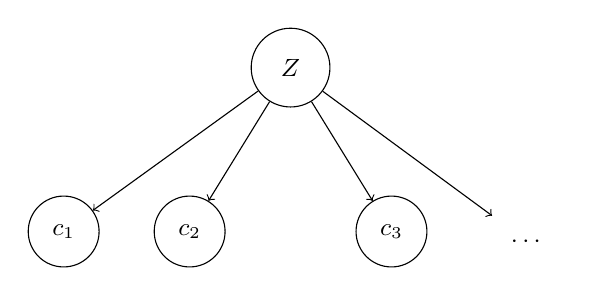
\begin{tikzpicture}[node distance=1.6cm, every node/.style={font=\small}]
\node (Z) [circle, draw, minimum size=1cm] {$Z$};
\node (c1) [circle, draw, minimum size=0.9cm, below left=1.4cm and 2.2cm of Z] {$c_1$};
\node (c2) [circle, draw, minimum size=0.9cm, below left=1.4cm and 0.6cm of Z] {$c_2$};
\node (c3) [circle, draw, minimum size=0.9cm, below right=1.4cm and 0.6cm of Z] {$c_3$};
\node (cn) [minimum size=0.9cm, below right=1.4cm and 2.2cm of Z] {$\cdots$};
\draw[->] (Z) -- (c1);
\draw[->] (Z) -- (c2);
\draw[->] (Z) -- (c3);
\draw[->] (Z) -- (cn);
\end{tikzpicture}
\caption{The graphical model shared by every curriculum considered in this paper. A latent state $Z$ generates several observation channels $c_1,\ldots,c_n$; the object of interest is never a mapping between channels, $c_i \to c_j$, but the fan-out structure through which each channel constrains the others only by way of $Z$. Basque case marking and verbal agreement, an image and its caption, and vision and proprioception during a reaching movement are all instances of this one diagram, differing only in how many arrows leave $Z$ and how corrupted each is.}
\label{fig:latent}
\end{figure}
 Under this description, a single-channel curriculum such as English-first pretraining supplies one view of $Z$; a two-channel curriculum such as Basque's case-and-agreement marking supplies two; a many-channel curriculum such as a signed utterance or an embodied interaction supplies as many as the language or the environment provides articulators and sensors.

The linearization of experience in written text, which is often stated as an intuitive objection to text-first training, receives its precise form here. Text is not deficient because it is linear. It is deficient because it supplies one view: whatever a linear encoding fails to preserve is unrecoverable, since there is no second view against which the first could be checked.

\subsection{Constraint Diversity}

The quantity of interest is not the number of channels but the extent to which they constrain one another through the latent state. Two channels constrain each other usefully when their agreement is caused by $Z$ rather than by anything shallower. This is the interaction information, and we define the constraint diversity of a curriculum stage as its sum over channel pairs:
\[
D(C)=\sum_{i<j}\Big[\,I(c_i;c_j)-I(c_i;c_j\mid Z)\,\Big].
\]
The first term measures how much the channels agree; the second removes agreement that survives conditioning on $Z$, which is agreement carrying no information about the state. Under the conditional independence assumed above the second term vanishes and $D$ reduces to the summed pairwise mutual information among channels, which is the clean case and the one the following sections use.

This definition behaves correctly at both extremes. A single-channel curriculum yields an empty sum and $D=0$: there is nothing to reconcile. A two-channel curriculum, of which Basque's redundant marking is the running example, yields one nonvanishing pair. Many-channel curricula yield correspondingly more. It is important that $D$ rewards rather than penalizes redundancy among channels, since redundancy is the mechanism Eichler identifies and any measure that treated overlapping channels as wasteful would be measuring the wrong thing.

\subsection{Non-Substitutability}

Constraint diversity as defined is necessary but not sufficient, and the reason is worth stating explicitly because it is the first objection a reader will raise. Duplicating a text corpus produces two channels with maximal mutual information and therefore high $D$, while teaching the learner nothing, because the mapping from one channel to the other is the identity and can be satisfied without representing $Z$ at all.

What distinguishes Basque from duplication is that recovering verbal agreement from case marking requires reconstructing the predicate-argument relation itself. The channels are mutually predictable only by way of the latent state. We therefore impose a minimality condition: $Z$ must be the simplest variable rendering the channels conditionally independent. If some simpler variable $W$ screens off the correlation between $c_i$ and $c_j$, the constraint is a surface regularity and the redundancy is spurious. A useful supplementary condition requires each channel to carry information the others do not,
\[
I(Z;c_i\mid C_{-i})>0,
\]
which excludes channels that are decorative rather than constraining. Together these conditions state formally what it means for a curriculum to supply views that must be reconciled rather than views that can be memorized against one another.

\subsection{Constraint Diversity Is Not the Whole Story}

One class of structure that intuitively belongs to any account of good foundational curricula is not measured by $D$, and the omission should be stated rather than left for a reader to find. Arabic root-and-pattern morphology distributes meaning across a consonantal root carrying semantic field and a vocalic template carrying morphosyntactic category. The two are separately observable and jointly determine the surface form, but they are close to independent: the root does not predict the template and the template does not predict the root. Constraint diversity as defined therefore assigns Arabic a low value despite a structure that is obviously consequential for a learner.

What such a system supplies is not redundancy but factorization: a product structure in which two axes of meaning are separately manipulable, which is the property the disentanglement literature has pursued under other names. Factorization and constraint diversity are distinct desiderata, and a curriculum can supply either without the other. We do not attempt to unify them here, and we note that the explicitness-diversity plane developed below is for that reason a projection of a larger space rather than a complete account. A further consequence is worth recording for implementers: non-concatenative morphology of this kind is the least favorable case for subword tokenization built on contiguity, since the root is discontinuous in the surface string.

\subsection{Measurement}

Since $Z$ is unobserved, $D$ is not directly computable, which would be fatal to any falsification criterion stated in terms of it. The conditional independence assumption provides the route around this. Training a predictor from one channel to another and measuring achievable accuracy lower-bounds $I(c_i;c_j)$ without requiring access to the latent state, and the sum of cross-modal predictability over channel pairs therefore serves as an empirical estimate of constraint diversity. This estimate is available before any model whose geometry is under test has been trained, which gives the present proposal a property Eichler's does not claim: the independent variable can be characterized in advance of the experiment rather than inferred from its outcome.

\subsection{The Explicitness-Diversity Plane}

Every foundational curriculum can now be located by two coordinates. Let $E$ denote symbolic explicitness, the degree to which relations are marked overtly rather than left to inference, which is the quantity Eichler's program maximizes. Let $D$ denote constraint diversity as defined above. Each curriculum occupies a point $(E,D)\in\mathbb{R}^2$.

\begin{table}[h]
\centering
\begin{tabular}{lcc}
\hline
\textbf{Curriculum} & $E$ & $D$ \\
\hline
English text & low & zero \\
Basque & high & low but nonzero \\
Synthetic logical language & maximal & low \\
American Sign Language & medium & high \\
Embodied multimodal interaction & medium & very high \\
Synthetic embodied substrate & maximal & maximal \\
\hline
\end{tabular}
\caption{Foundational curricula located by symbolic explicitness and constraint diversity.}
\label{tab:ed-plane}
\end{table}

The placement of Basque in this table deserves comment, since it corrects a framing that the discussion of Section~\ref{sec:convergent} might otherwise invite. Basque is not a purely $E$-axis intervention. Its double marking of predicate-argument structure supplies two mutually constraining encodings and therefore raises $D$ above the value for English text, even though both are delivered through a single written modality. Eichler's proposal was thus already partly a movement along the diversity axis, without being described in those terms. This is the strongest available evidence that the present paper extends his argument rather than opposing it: the property he isolated as mechanistically important is a $D$-axis property, and what follows is the observation that this axis extends much further than a single channel permits.

The two research programs now appear as optimizations over different coordinates. Eichler's trajectory, from English through Basque to a synthetic logical language, is approximately $\max E$. The trajectory proposed here, from text through speech and signed language to embodied interaction, is approximately $\max D$. Neither subsumes the other, and the plane makes visible that a curriculum can be maximal in one coordinate while remaining low in the other: a perfectly explicit synthetic language supplies one unambiguous view and therefore nothing to reconcile, while ordinary embodied experience supplies many views of relations none of which is marked overtly. The synthesis, in which every semantic relation is simultaneously encoded through explicit symbolic structure, perception, and action, occupies the upper right corner and is developed in neither paper.

\subsection{The Curriculum Functional and the Falsification Criterion}

A curriculum is a sequence of stages $\Gamma=(C_1,\ldots,C_T)$, and Eichler's hypothesis of a functional analogue to critical periods implies that constraint diversity is worth more early than late. This yields an objective
\[
\Gamma^{*}=\arg\max_{\Gamma}\int_{0}^{T} D(C_t)\,w(t)\,dt,
\]
with $w(t)$ decreasing, though we regard this as a statement of what the design problem is rather than as an objective anyone is presently in a position to optimize.

The empirical claim can be stated sharply. Let $F$ denote a measure of foundational representational quality, assessed through the geometric instruments described in the following section rather than through downstream benchmark performance alone. The null hypothesis is
\[
H_0:\quad \frac{\partial F}{\partial D}=0,
\]
that foundational constraint diversity has no measurable effect on representational geometry. The Representational Constraint Hypothesis predicts $\partial F/\partial D>0$ over some range, with saturation or decline beyond an optimal value, the latter expected on the basis of the non-monotonic dose effects reported for formal-language pre-pretraining. The hypothesis is falsified if curricula differing substantially in $D$, with architecture, total data, and downstream training held fixed, produce representational geometries that do not measurably differ.


\section{Compression Is Not the Objective}
\label{sec:compression}

An account of what makes representations good has been operating in the background of this literature for long enough that it is rarely stated, and it is in tension with the hypothesis developed here. The account holds that a representation improves as it becomes more compressed: that learning is the discovery of shorter descriptions, that the information bottleneck view of deep networks describes what training is for rather than merely what it sometimes does, and that interpretability is served by representations which are sparser and more economical than the ones a network arrives at on its own. The intuition is that brevity is evidence of understanding, since only a system that has found the structure can afford to discard everything else.

The intuition is not wrong so much as it identifies the wrong invariant. What matters about a representation is not how short it is but which distinctions it preserves. Description length and distinguishing capacity are related, and under favorable assumptions a perfectly compressed encoding preserves everything that can be distinguished. But those assumptions are demanding, and they are not obviously satisfied by distributed representations in trained networks, where features are superposed and no clean correspondence between code length and preserved distinction is guaranteed. Two representations of identical size may preserve very different distinctions, and a shorter representation that has collapsed a distinction the task requires is worse, not better, however economical it looks.

This bears directly on the present proposal because a curriculum satisfying many consistency constraints will tend to produce representations that are less compressed in the single-channel sense. A latent organized so that vision, proprioception, and text can all be rendered from it must retain structure that any one of those channels alone would be free to discard. Judged as a code for text it is wasteful. Judged by preserved distinguishing capacity it is richer, and the distinctions it retains are exactly the ones no single channel constrains on its own. The constraint diversity of Section~\ref{sec:constraint} can therefore be read in distinction-theoretic terms: a channel earns its place in a curriculum insofar as it preserves distinctions the other channels collapse, and the reconciliation the hypothesis requires is what prevents any one channel's collapses from becoming the representation's collapses.

\subsection{Why Learning Trajectories Are Not Monotonic in Simplicity}

The compression account also predicts the wrong shape for curricula, and the discrepancy is worth drawing out because it explains an empirical result the field currently records without explaining.

Deliberately simplified environments are pervasive wherever learners are engineered rather than merely observed. Pedagogical materials strip away variation that a competent adult handles without noticing. Standardized building components constrain constructed environments to a small set of regular shapes. Roads are made straight and uniform in part to compensate for the limited suspension of the vehicles that use them. In each case simplification is a scaffold matched to the current capacities of a learner or a mechanism, and in no case is the simplified version more true than what it replaced. It temporarily sacrifices richness in order to preserve the distinctions the learner is presently able to acquire.

The corollary is that scaffolds expire. Once a learner is no longer acquiring anything from a fixed regime, the variety of the environment has to be increased or learning stalls, and the increase is an increase in complexity rather than a further compression. Problem solving shows the same non-monotonicity at a shorter timescale, since a problem often has to be lifted into a higher-dimensional description before a simpler solution becomes reachable at all. Trajectories that produce competence are therefore not monotonic in simplicity, and a theory that identifies progress with compression progress has no natural way to accommodate the phases in which complexity must rise.

This supplies a reading of the non-monotonic dose curve reported for formal-language pre-pretraining, where benefit reverses beyond an optimal duration. On a compression account the reversal is anomalous, since more structured and more compressible early data ought not to become harmful by being extended. On the account given here it is expected: a low-variety substrate is a scaffold, it does its work while the distinctions it preserves are the ones still being acquired, and past that point it withholds the variety that further learning requires. The prediction generalizes beyond formal languages to any foundational phase, including the embodied phases proposed in this paper, and it is why Section~\ref{sec:experiment} varies the duration of that phase rather than fixing it.


\section{Experimental Design}
\label{sec:experiment}

The preceding section defined the independent variable. This section specifies how it would be varied and what would be measured, and it borrows Eichler's instruments deliberately: where the two proposals can be assessed on the same measurement axis, the results become commensurable rather than merely analogous, and the question of whether explicitness or diversity dominates becomes answerable rather than rhetorical.

\subsection{The Family of Conditions}

The design compares otherwise identical multimodal transformers whose foundational training stages differ only in constraint diversity, with architecture, parameter count, total token budget, and all subsequent training held fixed. A tractable version is available at the one to three billion parameter scale, matching the scale Eichler proposes for the Basque First experiment and permitting direct comparison of results.

The conditions form an ordered family rather than a binary contrast. A text-only condition supplies a single channel and serves as the $D=0$ baseline. A speech-and-text condition adds an acoustic channel constraining the same lexical content. A signed-language condition supplies the several partially predictive channels described in Section~\ref{sec:gestural}. An embodied condition supplies synchronized vision, pose, manipulation, and proprioception over shared physical episodes. Each condition is characterized in advance by the cross-modal predictability estimate of Section~\ref{sec:constraint}, so that the conditions are located on a continuous axis rather than merely labelled, and the analysis can regress representational outcomes on measured $D$ instead of on condition identity.

Two controls are essential. A duplicated-channel condition, in which a second channel is a transformation of the first that does not require the latent state to recover, tests the non-substitutability condition directly: it has high nominal channel count and high pairwise mutual information but should produce no representational benefit if the minimality argument of Section~\ref{sec:constraint} is correct. A matched-compute control equalizes the effective information volume across conditions, since multimodal channels are not free and an apparent diversity effect could otherwise reflect a difference in total signal.

Following Eichler's treatment of catastrophic forgetting, the transition into the shared text corpus is interleaved rather than abrupt, with a retained fraction of the foundational distribution throughout, since the adjacent literature indicates that early structure survives distribution shift only under such schedules. Since the foundational phase is expected to have an optimal duration rather than a monotonic benefit, on the pattern of the dose curve reported for formal-language pre-pretraining, the duration of that phase is varied within at least one condition rather than fixed by assumption.

\subsection{Measuring Foundational Geometry}

The quantity $F$ of the falsification criterion is representational rather than behavioral, and it is measured before downstream fine-tuning. Benchmark performance is reported, but it is not the primary evidence, for the reason Eichler gives: aggregate task performance can converge across curricula whose internal organization differs, so a design that measures only performance cannot detect the effect either paper predicts.

Four measurements are proposed. The Jacobian lens of Gurnee et al. (2026) identifies the sparse subspace of verbalizable representations, and the prediction is that its organization of structural and relational concepts varies systematically with $D$ in ways that correlate with downstream reasoning. Using this instrument matters beyond convenience: it is the same instrument Eichler proposes, applied across a different family of curricula, which places both experiments in one measurement space. Centered kernel alignment and representational similarity analysis compare latent geometry across conditions directly, testing whether high-$D$ curricula converge on shared organization that low-$D$ curricula do not. Probing classifiers measure what is linearly recoverable from foundational representations, with persistent objects, spatial relations, and event structure as the targets the hypothesis expects to become more accessible as $D$ increases. Finally, attention-head specialization is measured in the manner Eichler proposes for positional against morphological-semantic heads, with the embodied analogue being the ratio of within-modality heads to cross-modal binding heads in early layers.

\subsection{Reconstruction as a Direct Test}

The instruments described above are borrowed from interpretability research and inherit its dependencies: fitted lenses, trained probes, and a commitment to particular notions of what counts as structure. A further measurement is available that depends on none of this, follows directly from the definition of the hypothesis, and is cheap enough to run without access to substantial compute.

If a representation is organized around invariants that persist across channels, then a channel withheld from the model at test time should be recoverable from the remaining ones through that representation. If instead the model has learned channel-specific representations joined by translation, recovery should degrade sharply when the channel being predicted was not among the model's inputs during the episode in question. Held-out channel reconstruction therefore measures the property the hypothesis actually asserts, rather than a correlate of it, and it does so without requiring the reconstruction to be perceptually accurate: what is being tested is whether the latent retains the distinctions the withheld channel would have supplied, which a coarse reconstruction is sufficient to reveal.

This measurement composes with the depth-of-binding prediction of Section~\ref{sec:early}. Reconstruction from early-layer representations should be possible in models trained under constraint from the outset and should fail in models that acquired the constraint late, since in the latter case the information needed to reconstruct the withheld channel is present only above the layer where translation occurs. The pair of measurements is more informative than either alone, and neither requires downstream task training to interpret.

\subsection{Distinguishing the Two Axes}

The design admits a further condition that neither paper alone motivates and that constitutes the sharpest available test of the explicitness-diversity distinction. Holding $D$ fixed, vary $E$: compare an embodied curriculum whose linguistic channel is ordinary text against one whose linguistic channel is morphologically explicit in Eichler's sense. Holding $E$ fixed, vary $D$: compare a morphologically explicit single-channel curriculum against the same linguistic material accompanied by synchronized perceptual channels.

If the two axes contribute independently, their effects on $F$ should be approximately additive. If explicitness substitutes for diversity, the second comparison should show diminishing returns at high $E$, which would support the view that an unambiguous single channel leaves nothing to reconcile and that Eichler's synthetic substrate might therefore forfeit the property he identified as mechanistic. If diversity substitutes for explicitness, the first comparison should show diminishing returns at high $D$. All three outcomes are informative, and only the joint design can distinguish them, which is an argument for running the two proposals as one experimental program rather than as competing ones.

\subsection{Data}

The objection that terminates most embodied-curriculum proposals is availability, and it is the counterpart of the corpus problem Eichler addresses with the disambiguation cascade. His solution is instructive in form: rather than seeking a large native corpus, he constructs one by passing existing content through a transformation that forces structural resolution, on the reasoning that ambiguity cannot survive the crossing into a language that requires the relevant distinctions to be marked.

The embodied analogue is a rendering cascade. Text descriptions of physical situations can be passed through simulation or animation, which cannot render a described scene without resolving spatial relations, object extents, contact, and temporal ordering that the text left implicit. What returns is a synchronized second channel constraining the same content, generated at the scale of the text corpus rather than the scale of available motion capture. Existing sources supply the remainder: video with extracted pose, teleoperation and robot demonstration logs, and signed-language corpora with annotation.

Eichler's honesty about the limits of his cascade transfers directly and should be reproduced rather than elided. His semantic origin problem, that a cascade-derived corpus carries the conceptual distribution of its English source however thoroughly its morphology is resolved, has an exact counterpart here: a simulation-derived channel carries the priors of its simulator, and forced resolution is not guaranteed to be correct resolution. The corresponding control is likewise the same in form, a smaller condition trained on natively recorded embodied data, which tests whether the rendering cascade performs the structural work independently of the origin of its content. As in his design, either outcome is informative.


\section{The Unexplored Curriculum}
\label{sec:unexplored}

The explicitness-diversity plane contains a region that neither the Basque First proposal nor the present one develops, and identifying it is among the more consequential results of stating the two arguments in a common vocabulary.

Eichler's trajectory terminates in a synthetic training language: a constructed symbolic system encoding predicate-argument structure, evidentiality, quantifier scope, and entailment without the ambiguities of natural language, learnable by a network without needing to be usable by a person. The trajectory proposed here terminates in embodied multimodal curricula whose structure is distributed across perception and action. Stated as coordinates, one program maximizes explicitness while leaving diversity low, and the other maximizes diversity while leaving explicitness at whatever level natural channels happen to supply. The upper right corner of the plane is occupied by neither.

What would occupy it is a synthetic embodied substrate: a constructed system in which every semantic relation is encoded simultaneously through explicit symbolic marking, through perceptual structure, and through action, with the encodings mutually recoverable but separately observable. Such a substrate would be explicit in Eichler's sense, since nothing would be left to pragmatic inference, and diverse in the sense developed here, since each relation would be constrained several times over through channels that are not transcriptions of one another. Its construction is a research program rather than a design exercise, and the requirement that the symbolic and perceptual encodings be genuinely non-substitutable is likely to be its central difficulty, since a symbolic marking that can be read off a perceptual channel by a simple mapping would fail the minimality condition of Section~\ref{sec:constraint}.

The existence of this corner has an implication for how the two proposals should be read. If explicitness and diversity were substitutes, the corner would be redundant and one program would suffice. That they can be varied independently, and that a curriculum can be maximal in one coordinate while remaining low in the other, indicates that neither program subsumes the other and that the interesting object lies where they meet. This is a stronger relationship than complementarity: it means the experiment proposed in Section~\ref{sec:experiment} is not a contest between two hypotheses but the joint measurement that the construction of such a substrate would require.

\section{What We Do Not Know}
\label{sec:unknown}

The argument of this paper is a sequence of proposals, and its empirical content is entirely prospective. Several things are unknown, and the paper is worth less if they are not stated plainly.

We do not know whether foundational constraint diversity has any measurable effect on representational geometry. This is the hypothesis, and the design of Section~\ref{sec:experiment} is arranged so that it can fail. Aggregate benchmark performance may converge across curricula whose foundational geometry differs, in which case the effect exists but is invisible to standard evaluation, or the geometries may not measurably differ at all, in which case the hypothesis is false.

We do not know whether early structure survives the volume of later text training. This is the open question Eichler names for his own proposal, and it applies here without modification. The adjacent evidence is double-edged: early structure appears fragile under distribution shift, while interleaving demonstrably mitigates the loss. A curriculum that establishes cross-modal organization and then trains extensively on a single channel may retain that organization or may overwrite it, and the answer is not currently known for either proposal.

We do not know whether constraint diversity can be measured reliably in practice. The estimator of Section~\ref{sec:constraint} lower-bounds pairwise channel predictability with a learned predictor, and such estimates are sensitive to the capacity of the predictor and to the representation in which the channels are expressed. Whether the ordering of curricula by estimated diversity is stable under those choices is an empirical question that must be settled before the falsification criterion can be applied.

We do not know whether explicitness and diversity are independent, substitutes, or antagonists. The factorial design is proposed precisely because the answer is not evident from either paper's argument, and one possible outcome, diminishing returns from diversity at high explicitness, would tell against the position taken here.

We do not know the optimal duration of a foundational embodied phase, and there is reason from the formal-language literature to expect a non-monotonic dose response rather than a monotonic benefit. We also do not know whether embodied data generated through a rendering cascade carries structural distortions of its own, in the way that translated corpora carry translationese, and the native-data control of Section~\ref{sec:experiment} is included because that possibility cannot be dismissed by argument.

This is a case for a research direction rather than a report of results. The results do not exist.

\section{Conclusion}
\label{sec:conclusion}

The Basque First hypothesis proposes that curriculum order shapes foundational representational geometry, and identifies redundancy, the requirement that two encodings of one relation be reconciled, as the property that makes a curriculum consequential. This paper has argued that the property so identified is not specific to morphology, to language, or to symbolic channels of any kind, and that stating it in channel-neutral terms yields a design space in which the Basque First proposal and embodied curricula appear as optimizations of different coordinates rather than as rival claims about what should come first.

The resulting view of curriculum design is that its object is neither a language nor a modality but a set of consistency constraints: what a learner is required to reconcile during the period when its representational geometry is being established. American Sign Language is instructive in this framing not because it is a better language but because it demonstrates that a fully grammatical system can distribute one relation across several mutually constraining channels, and embodied interaction is instructive because it does the same without requiring language at all.

The central design variable of a foundational curriculum may therefore be neither language nor modality but the consistency constraints imposed during the period in which a model first learns to organize its latent representations. Whether that variable proves more important than symbolic explicitness, or complementary to it, is an empirical question, and the curriculum that would settle it has not been built. The framework presented here is intended to make the question precise enough to be worth building for.


\section{Related Work}
\label{sec:related}

The thesis of this paper, that foundational representations are organized by the consistency constraints imposed across partially independent observation channels, intersects several traditions in machine learning and cognitive science. The literature below is organized by the mechanism each tradition posits for representational quality rather than by surface domain, and each subsection closes by stating where the present framework diverges.

\subsection{Information-Theoretic and Compression Accounts}
\label{sec:rel-compression}

A dominant paradigm frames representation learning as the pursuit of minimal, highly compressed descriptions of sensory input. The information bottleneck principle \cite{tishby2000information} holds that an optimal representation maximizes information about a target while discarding everything else about the input; variational and minimum-description-length accounts of representation learning \cite{rissanen1978modeling, hinton1993keeping, kingma2013auto} treat learning as the discovery of shorter codes for the same reason.

These accounts explain feature selection well in single-channel, task-specific settings, but they identify compression itself as the objective. Section~\ref{sec:compression} argues that compression cannot distinguish a representation that has found genuine structural invariants from one that has collapsed a task-relevant distinction to satisfy an inductive bias toward brevity. The present framework diverges by measuring representational value through preserved distinguishing capacity across channels rather than through description length within one channel; the constraint diversity $D(C)$ of Section~\ref{sec:constraint} is in this sense the opposite of a compression objective, since it is maximized by retaining exactly the structure a single-channel code would discard as redundant.

\subsection{Contrastive and Multimodal Alignment}
\label{sec:rel-contrastive}

Multimodal pretraining methods, among them CLIP \cite{radford2021learning}, ALIGN \cite{jia2021scaling}, and self-supervised contrastive frameworks such as SimCLR \cite{chen2020simple} and VICReg \cite{bardes2021vicreg}, use cross-view agreement as an explicit training objective, forcing representations of paired observations toward a shared space through contrastive loss or variance-covariance regularization.

These methods demonstrate empirically that cross-channel agreement produces useful representations, but they are developed and evaluated as techniques for transferable features and retrieval rather than as a general theory of foundational curricula, and they operate almost entirely on pairwise, static projections rather than the $n$-channel curricula this paper considers. The present work treats their shared mechanism as an instance of a general principle rather than a technique specific to vision and text, and asks when in training that mechanism should be applied rather than only how.

\subsection{Curriculum Learning and Pretraining Data Ordering}
\label{sec:rel-curriculum}

Curriculum learning in its classical form, introduced by Elman's account of the advantages of starting small \cite{elman1993starting} and formalized by Bengio et al. \cite{bengio2009curriculum}, sequences examples by difficulty within a fixed data distribution. This is a different variable from the one considered here, since it concerns pacing rather than the number of channels a curriculum supplies. Controlled studies varying only the order of pretraining data find that ordering reshapes learning trajectories and representational geometry even where final loss converges \cite{dini2026impact}, which is the dissociation between geometry and aggregate performance that motivates measuring representational quality directly in Section~\ref{sec:experiment} rather than through benchmark scores alone.

A separate line establishes that non-linguistic structure transfers to language modeling. Papadimitriou and Jurafsky \cite{papadimitriou2020learning} show that pretraining on music, code, and nested symbolic sequences transfers structural bias to subsequent language modeling. Hu et al. \cite{hu2025formal} show that pre-pretraining on formal languages with hierarchical structure improves natural-language learning, with structured tokens outperforming natural ones and with benefit reversing beyond an optimal duration. Shinnick et al. \cite{shinnick2025procedural} find that pretraining on procedural data yields modular internal structure for algorithmic reasoning.

We build on this tradition but propose a unified mechanism: these substrates succeed not because of domain-specific properties but because of the constraint structure they impose during a period when a shortcut solution is not yet available, the argument developed in Section~\ref{sec:early}. Where this literature treats formal or structured pretraining as a special case, we treat it as one point in a space also containing multimodal and embodied curricula, and introduce the explicitness-diversity plane of Section~\ref{sec:constraint} to separate symbolic clarity from cross-channel reconciliation as distinct curriculum variables.

\subsection{Embodied, Grounded, and Robot Foundation Models}
\label{sec:rel-embodied}

Grounded cognition holds that abstract concepts remain organized around modal, sensorimotor structure \cite{barsalou1999perceptual, lakoff1980metaphors}, a position engaged directly in Section~\ref{sec:development}. In artificial intelligence this perspective has motivated embodied foundation models and vision-language-action architectures, including RT-2 \cite{brohan2023rt2}, PaLM-E \cite{driess2023palme}, and the Open X-Embodiment effort \cite{padalkar2023open}, which integrate camera views, proprioception, and action into a shared model.

These systems treat embodiment as an application domain, a necessary interface to physical hardware, rather than as a candidate foundational substrate; embodied data is typically introduced through fine-tuning or co-training alongside a text-pretrained backbone rather than as the initial curriculum. On the account of Section~\ref{sec:early}, introducing multi-channel physical constraints after a competent text-only representation already exists is exactly the condition under which the Translation Shortcut Hypothesis predicts a superficial mapping rather than structural reorganization. The present proposal differs by treating embodied interaction as a candidate foundational stage rather than a downstream application, and by making that difference an experimentally testable claim rather than a design preference.

\subsection{Sign Language Linguistics}
\label{sec:rel-typology}

Sign language linguistics, from Stokoe's original demonstration that ASL has phonological structure \cite{stokoe1960sign} through subsequent work establishing its grammatical use of space, non-manual marking, and simultaneous articulation \cite{sandler2006sign}, provides the linguistic grounding for Section~\ref{sec:gestural}. Machine learning treatments of signed language have concentrated on translation, glossing, and recognition pipelines \cite{camgoz2018neural, koller2019weakly} rather than on signed language's significance as a curriculum, and its status as a naturally occurring, high-diversity, fully grammatical instance of the mechanism this paper describes has not, to our knowledge, been previously stated.

\subsection{The Basque First Hypothesis}
\label{sec:rel-eichler}

The closest precedent to the present proposal is Eichler's Basque First hypothesis \cite{eichler2026basque}, discussed at length in Sections~\ref{sec:convergent} through~\ref{sec:constraint} rather than summarized again here. Eichler identifies the redundant encoding of predicate-argument structure in Basque, case marking on the noun together with polypersonal agreement on the verb, as a consistency constraint rather than a distributional cue, and proposes this as the mechanism by which curriculum order shapes foundational representational geometry. The present paper takes that identification as established within its domain and generalizes it beyond a single written channel; the extent of the debt and the point of divergence, the distinction between symbolic explicitness and constraint diversity as separate curriculum objectives, are stated in full in Section~\ref{sec:constraint} and are not restated here.


\begin{thebibliography}{99}

\bibitem{alemi2016deep}
Alexander A. Alemi, Ian Fischer, Joshua V. Dillon, and Kevin Murphy.
\newblock Deep variational information bottleneck.
\newblock \emph{arXiv preprint arXiv:1612.00410}, 2016.

\bibitem{bardes2021vicreg}
Adrien Bardes, Jean Ponce, and Yann LeCun.
\newblock VICReg: Variance-invariance-covariance regularization for self-supervised learning.
\newblock \emph{arXiv preprint arXiv:2105.04906}, 2021.

\bibitem{barsalou1999perceptual}
Lawrence W. Barsalou.
\newblock Perceptual symbol systems.
\newblock \emph{Behavioral and Brain Sciences}, 22(4):577--609, 1999.

\bibitem{bengio2009curriculum}
Yoshua Bengio, J\'{e}r\^{o}me Louradour, Ronan Collobert, and Jason Weston.
\newblock Curriculum learning.
\newblock In \emph{Proceedings of the 26th International Conference on Machine Learning (ICML)}, 2009.

\bibitem{brohan2023rt2}
Anthony Brohan et al.
\newblock RT-2: Vision-language-action models transfer web knowledge to robotic control.
\newblock \emph{arXiv preprint arXiv:2307.15818}, 2023.

\bibitem{camgoz2018neural}
Necati Cihan Camg\"{o}z, Simon Hadfield, Oscar Koller, Hermann Ney, and Richard Bowden.
\newblock Neural sign language translation.
\newblock In \emph{Proceedings of the IEEE Conference on Computer Vision and Pattern Recognition (CVPR)}, 2018.

\bibitem{chen2020simple}
Ting Chen, Simon Kornblith, Mohammad Norouzi, and Geoffrey Hinton.
\newblock A simple framework for contrastive learning of visual representations.
\newblock In \emph{Proceedings of the 37th International Conference on Machine Learning (ICML)}, 2020.

\bibitem{dini2026impact}
Luca Dini, Lorenzo Domenichelli, Dominique Brunato, and Felice Dell'Orletta.
\newblock On the impact of pretraining data ordering in transformer encoder- and decoder-only language models.
\newblock \emph{Knowledge-Based Systems}, 2026.

\bibitem{driess2023palme}
Danny Driess et al.
\newblock PaLM-E: An embodied multimodal language model.
\newblock \emph{arXiv preprint arXiv:2303.03378}, 2023.

\bibitem{eichler2026basque}
David Eichler.
\newblock Curriculum order and the geometry of learned representations: The Basque First hypothesis.
\newblock \emph{Zenodo}, July 2026.
\newblock \url{https://doi.org/10.5281/zenodo.21396981}.

\bibitem{elman1993starting}
Jeffrey L. Elman.
\newblock Learning and development in neural networks: The importance of starting small.
\newblock \emph{Cognition}, 48(1):71--99, 1993.

\bibitem{hinton1993keeping}
Geoffrey E. Hinton and Drew van Camp.
\newblock Keeping the neural networks simple by minimizing the description length of the weights.
\newblock In \emph{Proceedings of the 6th Annual Conference on Computational Learning Theory (COLT)}, 1993.

\bibitem{hu2025formal}
Michael Y. Hu et al.
\newblock Between circuits and Chomsky: Pre-pretraining on formal languages imparts linguistic biases.
\newblock \emph{arXiv preprint arXiv:2502.19249}, 2025.

\bibitem{jia2021scaling}
Chao Jia et al.
\newblock Scaling up visual and vision-language representation learning with noisy text supervision.
\newblock In \emph{Proceedings of the 38th International Conference on Machine Learning (ICML)}, 2021.

\bibitem{kingma2013auto}
Diederik P. Kingma and Max Welling.
\newblock Auto-encoding variational Bayes.
\newblock \emph{arXiv preprint arXiv:1312.6114}, 2013.

\bibitem{koller2019weakly}
Oscar Koller, Necati Cihan Camg\"{o}z, Hermann Ney, and Richard Bowden.
\newblock Weakly supervised learning with multi-stream CNN-LSTM-HMMs to discover sequential parallelism in sign language videos.
\newblock \emph{IEEE Transactions on Pattern Analysis and Machine Intelligence}, 42(9), 2019.

\bibitem{lakoff1980metaphors}
George Lakoff and Mark Johnson.
\newblock \emph{Metaphors We Live By}.
\newblock University of Chicago Press, Chicago, 1980.

\bibitem{padalkar2023open}
Abhishek Padalkar et al.
\newblock Open X-Embodiment: Robotic learning datasets and RT-X models.
\newblock \emph{arXiv preprint arXiv:2310.08864}, 2023.

\bibitem{papadimitriou2020learning}
Isabel Papadimitriou and Dan Jurafsky.
\newblock Learning music helps you read: Using transfer to study linguistic structure in language models.
\newblock In \emph{Proceedings of the 2020 Conference on Empirical Methods in Natural Language Processing (EMNLP)}, 2020.

\bibitem{radford2021learning}
Alec Radford et al.
\newblock Learning transferable visual models from natural language supervision.
\newblock In \emph{Proceedings of the 38th International Conference on Machine Learning (ICML)}, 2021.

\bibitem{rissanen1978modeling}
Jorma Rissanen.
\newblock Modeling by shortest data description.
\newblock \emph{Automatica}, 14(5):465--471, 1978.

\bibitem{sandler2006sign}
Wendy Sandler and Diane Lillo-Martin.
\newblock \emph{Sign Language and Linguistic Universals}.
\newblock Cambridge University Press, Cambridge, 2006.

\bibitem{shinnick2025procedural}
Zachary Shinnick, Liangze Jiang, Hemanth Saratchandran, Anton van den Hengel, and Damien Teney.
\newblock Transformers pretrained on procedural data contain modular structures for algorithmic reasoning.
\newblock \emph{arXiv preprint arXiv:2505.22308}, 2025.

\bibitem{stokoe1960sign}
William C. Stokoe.
\newblock Sign language structure: An outline of the visual communication systems of the American deaf.
\newblock \emph{Studies in Linguistics: Occasional Papers}, 8, 1960.

\bibitem{tishby2000information}
Naftali Tishby, Fernando C. Pereira, and William Bialek.
\newblock The information bottleneck method.
\newblock \emph{arXiv preprint physics/0004057}, 2000.

\end{thebibliography}

\end{document}
